\documentclass[../../main.tex]{subfiles}

\begin{document}
Assuming the tree $T$ created above is approximately accurate, we now seek to infer genotypes from this phylogeny so as to overcome errors and noise associated with low coverage SCS data.
We first determine weights for attaching point mutations and different types of LOH events to different edges of the tree, and then use these weights to determine genotype probabilities for each cell.
The approximate phylogeny was found by combing information from across the genome, however to infer cell genotypes we shall return to considering individual loci.

\subsubsection*{SNV weights}
In the simplest case, we ignore any potential loss of heterozygosity.
For each edge of the tree $e$, we seek to answer the following question: assuming there is a point mutation at this locus, what is the probability it occurred at $e$?

To begin with, we compute the likelihood of all descendants of an edge in the tree having the same genotype.
We say that $\pi_0(e), \pi_1(e)$ and $\pi_2(e)$ are respectively the likelihoods that all descendants of $e$ are homozygous reference, heterozygous and homozygous alternate.

These values are taken to be
\begin{equation}
\pi_g(e) = \prod_{\{j:c_j\succ e\}} P(g_j = g)
\end{equation}
where $c_j\succ e$ indicates that the $j^{th}$ cell is below $e$ in $T$.
$P(g_j = g)$ here are the probabilities calculated in Equation~\eqref{eq:posteriorgenotypes}.
We also compute one more value, $\pi_\mu(e)$, defined as the likelihood that all descendants of $e$ have a genotype of either 1 or 2, that is to say they are mutant.
These four values can be computed recursively at each locus in $O(m)$ time by multiplying the corresponding values from the two branches directly beneath each branch.

If an SNV occurred at edge $e$ in $T$, we would expect that all descendants of $e$ would have genotypes of 1 or 2, while all other cells would have genotype 0 (assuming infinite sites).
Letting $\rho$ be the edge ancestral to all sampled cells, it is easy to verify that this likelihood simplifies to:
\begin{equation*}
    \prod_{c_x\succ e}P(g_x =1,2)\prod_{c_y\nsucc e} P(g_y = 0) = \pi_\mu(e)\frac{\pi_0(\rho)}{\pi_0(e)}
\end{equation*}
If a mutation occurred at a particular locus, the prior probability that it occurred on branch $e$ can be found by using the edge lengths of $T$: mutations occur on longer edges more frequently.
We must undo the Jukes-Cantor correction that was useful for neighbor joining to find a value proportional to the expected number of SNVs along an edge.
We find $\overline{p}_e = \frac{3}{4}\left(1-e^{-\frac{4}{3}d_e}\right)$ to be such a value and therefore define the prior probability (conditioned on the existence of a mutation at this locus) of attaching a SNV to edge $e$ to be:
\begin{equation*}
    P(S_e) = \frac{\overline{p}_e}{\sum_{e'}\overline{p}_{e'}}
\end{equation*}
Since $\pi_0(\rho)$ and $\sum_{e}\overline{p}_{e}$ are constant for a locus, we define a weight for attaching a SNV with no LOH to edge $e$ as:
\begin{equation*}
    W(S_e) = \frac{\pi_\mu(e)}{\pi_0(e)} \overline{p}_e
\end{equation*}
which is proportional to the posterior probability of attachment at $e$ up to a normalization constant (assuming a SNV occurred at this locus).
This is because the ratio $\pi_\mu/\pi_0$ is as a likelihood, where the `observations' are the posterior probabilities from the last stage of the algorithm, and $\overline{p_e}$ is proportional to a prior for $e$, conditioned on the site being mutant and $T$.

When we recurse up the tree computing $\pi_g$ values, we can also compute and store these weights $W(S_e)$.
If we recursively sum the weights from the two children of each node, at the root this sum value will equal the total sum of weights and we can thereafter derive the probabilities:
\begin{equation} \label{eq:SNVattachP}
    P(S_e\,\mid\,SNV,\,T) = \frac{W(S_e)}{\sum_{e'}W(S_e)}
\end{equation}


\subsubsection*{Weights for loss of heterozygosity}

\begin{figure}[H]
	\centering

	\begin{subfigure}{0.2\textwidth}
		\centering
		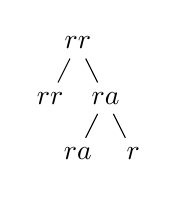
\begin{tikzpicture}[sibling distance=2em, level distance=2em]
  \node {$rr$}
    child { node {$rr$} }
    child { node {$ra$}
      child { node {$ra$} }
      child { node {$r$}}
          };
		\end{tikzpicture}
		\caption{Case 1}
	\end{subfigure}
	\begin{subfigure}{0.2\textwidth}
		\centering
		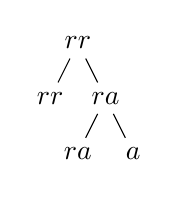
\begin{tikzpicture}[sibling distance=2em, level distance=2em]
  \node {$rr$}
    child { node {$rr$} }
    child { node {$ra$}
      child { node {$ra$} }
      child { node {$a$}}
          };
		\end{tikzpicture}
		\caption{Case 2}
	\end{subfigure}
	\begin{subfigure}{0.2\textwidth}
		\centering
		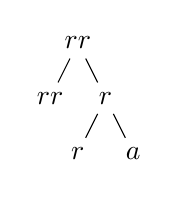
\begin{tikzpicture}[sibling distance=2em, level distance=2em]
  \node {$rr$}
    child { node {$rr$} }
    child { node {$r$}
      child { node {$r$} }
      child { node {$a$}}
          };
		\end{tikzpicture}
		\caption{Case 3}
	\end{subfigure}
	\begin{subfigure}{0.2\textwidth}
		\centering
		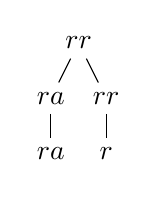
\begin{tikzpicture}[sibling distance=2em, level distance=2em]
  \node {$rr$}
    child { node {$ra$} 
    	child { node {$ra$} }
    	  }
    child { node {$rr$} 
    	child { node {$r$} }
    	};
		\end{tikzpicture}
        \caption{Case 4}
    \end{subfigure}
    \caption{Different ways loss of heterozygosity can occur in a tree. The LOH in case 4 is undetectable from the SCS reads and thus ignored.}
    \label{fig:treecases2}
\end{figure}

The more complicated cases involve both a SNV and a ploidy change occurring at the same locus.
The four possible ways this can occur is shown in Figure~\ref{fig:treecases2}.

For case 1, a point mutation occurred at edge $e_1$ before a ploidy change dropped the alternate allele at $e_2$.
We expect that all cells $e\succ e_2$ will have genotype 0, since the alternate allele has been dropped for this subclone.
Cells for which $e\succ e_1$ but $e\nsucc e_2$ will have genotype 1: these are the cells from the SNV subclone that did not experience the LOH.
All other cells will have genotype 0, as they are not in the subclone of the SNV.

Similar to the simplest case, the likelihood of a SNV at $e_1$ followed by a dropped alternate allele at $e_2$ is therefore given by:
\begin{equation*}
    \prod\limits_{c_x\succ e_2}P(g_x = 0)\times\prod\limits_{c_y\succ e_1,\nsucc e_2} P(g_y = 1)\times\prod\limits_{c_z\nsucc e_1, \nsucc e_2} P(g_z=0)
    = \pi_0(e_2)\cdot\frac{\pi_1(e_1)}{\pi_1(e_2)}\cdot\frac{\pi_0(\rho)}{\pi_0(e_1)}
\end{equation*}

The prior probability of attaching the SNV at $e_1$ is the same as in the simple case: normalized $\overline{p}_{e_1}$.
The prior probability of attaching a loss of heterozygosity at $e_2$, however, is subtly different.
We assume that a loss of heterozygosity affecting just a single cell is far less probable than an allelic dropout event during the amplification process.
Therefore we define
\begin{equation*}
    P(L_{e}) = \frac{\overline{p}_e}{\sum_{e'\in E-E_L}\overline{p}_{e'}}
\end{equation*}
where $E_L$ is the set of all edges directly above a leaf node.
This is the same as setting the prior probability of a loss of heterozygosity affecting individual cells to 0.
The weight of attaching the SNV to $e_1$ and the LOH to $e_2\succeq e_1$ for case 1 is:
\begin{equation}
    W^{(1)}(S_{e_1},\,L_{e_2}) = \frac{\pi_0(e_2)\pi_1(e_1)}{\pi_1(e_2)\pi_0(e_1)}\overline{p}_{e_1}\overline{p}_{e_2}
\end{equation}
This is proportional to a joint posterior probability, conditioned on several assumptions: both a SNV and LOH have occurred at the locus; the SNV was ancestral to the ploidy change and the loss of heterozygosity dropped the alternate allele.
This weight can be converted into a joint attachment probability by normalizing over the pairs of edges for which $\{e_1,e_2\}\subset E-E_L$ and $e_1\preceq e_2$.

The weights for cases 2 and 3 can be found using similar logic to be:
\begin{equation}
    W^{(2)}(S_{e_1},\,L_{e_2}) = \frac{\pi_2(e_2)\pi_1(e_1)}{\pi_1(e_2)\pi_0(e_1)}\overline{p}_{e_1}\overline{p}_{e_2}
\end{equation}
\begin{equation}
    W^{(3)}(S_{e_1},\,L_{e_2}) = \frac{\pi_2(e_1)}{\pi_0(e_1)}\overline{p}_{e_1}\overline{p}_{e_2}
\end{equation}
although $W^{(3)}$ has the slightly different domain for normalization: $e_2\in E-L,\,e_1\in E$ and of course $e_1\succeq e_2$.

\subsubsection*{Marginal probabilities of ploidy change}

For cases 1 and 2, it will be useful to answer the following question at each edge: assuming there is a case $i$ event at this locus and a SNV has already been observed ancestral to this edge, what is the probability that a LOH event will happen at this edge?
Let us assume that an SNV occurs at this locus and that a case 1 loss of heterozygosity also definitely occurs.
This is to say that if an edge experiences a loss of heterozygosity the alternate allele must be dropped, and an ancestral SNV at this locus is implicit. 
We first see that for any $e'\preceq e$: 
\begin{align*}
    P^{(1)}(L_e\,\mid\,S_{\preceq e}) &= P(L_e\cap S_{\preceq e})\\
    &= P(L_e\cap(S_\rho \cup S_{e_i} \cup \dots)\\
    &= P((L_e\cap S_\rho) \cup (L_e\cap S_{e_i}) \cup \dots)
\end{align*}
Due to infinite sites, mutations on different branches at a locus are mutually exclusive, hence we can sum
\begin{equation*}
    P^{(1)}(L_e\,\mid\,S_{\preceq e}) \propto \sum_{e'\prec e}W^{(1)}(L_e, S_{e'}) + \frac{1}{2} W^{(1)}(L_e, S_e)
\end{equation*}

If the SNV and LOH happen on the same branch, on average we expect the SNV to occur halfway down the branch leaving only half the distance for a ploidy change to occur afterwards, hence the factor of $\frac{1}{2}$ for the second term.
The conditional probability is proportional to the term on the right up to a normalization factor.

This has all been shown assuming case 1 to be true for the locus, but the values for case 2 are exactly similar and can be computed at the same time.
Case 3, however, is somewhat different, as we need to find the probability of an LOH given that a SNV occurs in a descendant branch:
\begin{align*}
    P^{(3)}(L_e\,\mid\,\neg S_{\prec e}) &= P(L_e\cap S_{\succeq e})\\
    &\propto \sum_{e'\succ e}W^{(3)}(S_{e'},\,L_e) + \frac{1}{2}W^{(3)}(S_e,\,L_e)
\end{align*}
Again to return the true marginal probability these sums must be normalized sum over all valid pairs.

The marginal probabilities here have so far assumed not only that there is a SNV and loss of heterozygosity at the locus, but also that their particular case is true.
We established when determining prior probabilities for $\sigma$ that $P(\text{case }i\,\mid\,LOH,\,SNV) = 1/3$ for $i\in[0,3]$.
We take $P(LOH) = P(H)$ as an input parameter, and $P(SNV)$ for a locus can be given by the posterior distribution of $\sigma$ for the locus, where $P(SNV) = 1-P(\sigma=0)$.

\subsubsection*{Upwards-downwards algorithm}
The na\"ive approach for calculating these values would be to visit each edge in a tree traversal and from each edge retrieve all the values required from its ancestors or descendants.
If we consider $P^{(3)}(S_{L_e\,\mid\neg S_{\prec e}})$, however, at each edge $e$ we require the joint probability $P^{(3)}(S_{e'},\,L_e)$ using values from all the descendants of $e$ as well as a product of probabilities from all the ancestors of $e$.
The na\"ive approach has a total time complexity of $O(nm^2)$ which does not asymptotically increase the complexity of SCarborSNV, but nonetheless there is a more efficient algorithm using a dynamic programming approach.

We saw that $\pi_g(e)$ were useful values that could be found recursively in a single pass up the tree.
Similarly there are other sub-problem values we can store at each node so that we only need to make two passes of the tree to find our final phylogeny aware genotype probabilities.

In the first pass (upwards step) we store three values:
\begin{itemize}
    \item $\pi_g$ and $\pi_m$
        \begin{itemize}
            \item The value at $e$ is the sum of values from both children.
            \item The base case at the leaves is the original genotype posteriors.
        \end{itemize}
    \item $\sum_e W(S_e)$
        \begin{itemize}
            \item The value at $e$ is the sum from both children added to $W(S_e)$.
        \end{itemize}
    \item $\sum_{e'\succ e} \frac{\pi_2(e')}{\pi_0(e')}\overline{p}_{e'}$
        \begin{itemize}
            \item The value at $e$ is the sum from both children added to the term evaluated at $e$.
        \end{itemize}
\end{itemize}

Once the root has been reached, the value of $\sum W(S_e)$ can be used to normalize these $W$ values to $P(S_e)$ at each edge in the following steps.
In the second pass (downwards step) we compute the following partial sum by adding the value at $e$ to the partial sum of the parent:
\begin{itemize}
    \item $\sum_{e'\prec e}\frac{\pi_1(e')}{\pi_0(e')}\overline{p}_{e'}$
\end{itemize}

From these values we can calculate:
\begin{equation*}
    P^{*(1)}(S_{e'},L_e) = \left(\sum_{e'\prec e}\frac{\pi_1(e')}{\pi_0(e')}\overline{p}_{e'} + \frac{1}{2}\frac{\pi_1(e)}{\pi_0(e)}\overline{p}_e\right)\overline{p}_e\frac{\pi_0(e)}{\pi_1(e)}
\end{equation*}
Each time one of these sums is calculated in the downward pass we can add it to a global total.
The same is done for  cases 2 and 3.
These are the last remaining value required to calculate all edge probabilities: $P(S_e)$, $P^{(1)}(L_e\mid S_{\preceq e})$, $P^{(2)}(L_e\mid S_{\preceq e})$ and $P^{(3)}(L_e\mid \neg S_{\preceq e})$.

\begin{algorithm}
    \caption{Upwards-Downwards}
    \begin{algorithmic}[5]
        \Procedure{FillUpwards}{Node}\Comment{Recursive upwards pass}
        \If{Node is leaf}
            \State Node.$\pi_g \gets P(g_j = g,\mid\,D_i)$
            \State Node.$\pi_\mu \gets P(g_j=1,\mid\,D_i) + P(g_j=2,\mid\,D_i)$
            \State Node.$\sum W(S_e) \gets$ Node.$W(S_e) \gets \text{Node.}\pi_\mu\div \text{Node.}\pi_0\times\text{Node.}\overline{p}$ 
            \State Node.aux0 $\gets$ Node.$\pi_2\div\text{Node.}\pi_0\times\text{Node.}\overline{p}$
            \State Node.$\sum\text{aux0}\gets 0$\Comment{Auxiliary partial sum for calculating probabilities}
        \Else
            \State \Call{FillUpwards}{Child 1}\Comment{Recursive calls first}
            \State \Call{FillUpwards}{Child 2}
            \State Node.$\pi \gets$ Child 1.$\pi\times$ Child 2.$\pi$\Comment{For all four $\pi$ values}
            \State Node.$\sum W(S_e) \gets \text{Node.}W(S_e) + \text{Child 1.}\sum  W(S_e)+ \text{Child 2.}\sum W(S_e)$
            \State Node.aux0 $\gets$ Node.$\pi_2\div\text{Node.}\pi_0\times\text{Node.}\overline{p}$
            \State Node.$\sum\text{aux0} \gets \text{Child 1.}\sum\text{aux0} + \text{Child 1.aux0} + \text{Child 2.}\sum\text{aux0} + \text{Child 2.aux0}$
        \EndIf
        \EndProcedure
        \Procedure{FillDownwards}{Node}\Comment{Recursive downwards pass}
        \If{Node is root}
            \State Node.$\sum \frac{\pi_1}{\pi_0}\overline{p} \gets \frac{\pi_1}{\pi_0}\overline{p}$\Comment{Initialize sum at root}
            \State \textbf{global} $\sum W(S_e) \gets \text{Node.}\sum W(S_e)$\Comment{Used to normalize weights}
            \State Node.$P(S_e) \gets \text{Node.}W(S_e) \div \text{\textbf{global }} \sum W(S_e)$
            \State \Call{FillDownwards}{Child 1}
            \State \Call{FillDownwards}{Child 2}
        \Else
            \State Node.$\sum \frac{\pi_1}{\pi_0}\overline{p} \gets \text{Parent.}\sum \frac{\pi_1}{\pi_0}\overline{p} + \frac{\pi_1}{\pi_0}\overline{p}$
            \State Node.$P(S_e) \gets \text{Node.}W(S_e) \div \text{\textbf{global }} \sum W(S_e)$
            \If{Node is not leaf}
            \State \Call{FillDownwards}{Child 1}\Comment{Recursive calls last}
            \State \Call{FillDownwards}{Child 2}
            \EndIf
        \EndIf
        \EndProcedure
        \State \Call{FillUpwards}{Root}\Comment{Call both traversals to fill needed values}
        \State \Call{FillDownwards}{Root}
    \end{algorithmic}
\end{algorithm}


The upwards-downwards algorithm prepares the tree at each candidate locus for a final dynamic programming approach to call the final genotypes.

\subsubsection*{Genotyping cells}
%TODO got to keep a running probability of case 3, separate from genotype probs. prob of 2 from 0 = p(S_e)*(sum(P(case 3 ancestral))+case2 at e)
With all of these values computed for each of the edges in the tree, we can use a dynamic programming algorithm to genotype the cells. We complete a depth first traversal of the tree keeping track of genotype probabilities at every node. We also keep track of the probability $P(L_{\preceq e}^{(3)})$ that a silent case 3 haploid event has occured ancestral to each node. The initial conditions for the root node are the genotype probabilities $P(g=0)=1$ and $P(g=1)=P(g=2)$ and $P(L_{\preceq \rho}^{(3)}) = 0$. Let $n_1$ be the direct ancestor of $n_2$ such that $n_1$ and $n_2$ are joined by $e$ and have genotypes $g_1$ and $g_2$ respectively. Therefore we define the relations:
%TODO write these including P(SNV) and P(LOH)
%TODO also instead of just probability of silent mutation, have conditional probability of case 3 given g=0, therefore keep track of separate haploid 0 genotype
\begin{equation*}
P(L^{(3)}_{\preceq n_2}) = P(L^{(3)}_{\preceq n_1}) +P(L^{(3)}_e)
\end{equation*}
\begin{align*}
P(g_2 = 0) = &P(g_1=0)\left[(1-P(S_e))+P(S_e)P(L^{(1)}_e)\right]\\
+ &P(g_1 = 1)\left[P(L^{(1)}_e)\right]
\end{align*}
%TODO is it necessary to include that no type 3, is that assumed?
\begin{align*}
P(g_2 = 1) = &P(g_1=0)\left[P(S_e)(1-P(L^{(1)}_e)-P(L^{(2)}_e))\right]\\
+ &P(g_1 = 1)\left[1-P(L^{(1)}_e)-P(L^{(2)}_e)\right]
\end{align*}
%TODO do we need 1-P(S_e) here?
\begin{align*}
P(g_2=2) = &P(g_1=0)\left[P(S_e)(P(L^{(3)}_{\preceq n_2}) + P(L^{(2)}_e))\right]\\
+ &P(g_1=1)\left[P(L^{(2)}_e)\right]\\
+ &P(g_1=2)
\end{align*}

When the tree traversal reaches the leaf nodes, these are taken to be the cell genotype probabilities. The cell will be genotyped in accordance with the highest probability.


\end{document}
